\begin{center}
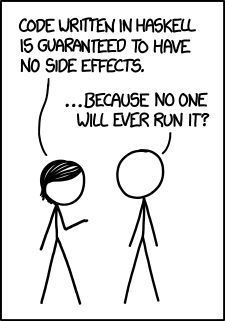
\includegraphics[width=0.3\textwidth]{haskell-1312.png}
\end{center}
\begin{center}
\url{http://xkcd.com/1312/}
\end{center}

\section{Über die Programmiersprache}
\citeauthor{lyahfgg} beschreibt in der Einleitung zu \autocite{lyahfgg} 
Haskell wie folgt:

Haskell ist eine \emph{rein funktionale} Programmiersprache.
Im Gegensatz zu \emph{imperativen} Programmiersprachen, bei denen man dem
Computer eine Folge von ausführbaren Aufgaben übergibt (Strukturen, die diesen
Ablauf steuern, wären beispielsweise ħforħ und ħwhileħ), bestehen Programme in
rein funktionalen Sprachen aus einer Menge von Funktionsdefinitionen, die man
als Abbildungen von Eingabedaten auf Ausgabedaten verstehen kann.

Möchte man beispielsweise die Fakultät einer Zahl berechnen, so gibt man in
einer imperativen Sprache die konkret notwendigen Anweisungen, um die
Fakultät eines Eingabedatums zu berechnen; in einer rein funktionalen Sprache
definiert man dagegen die Fakultät als rekursive Abbildung folgendermaßen:
\[ \_!:\ \funcdef{ \N &\to& \N \\ n &\mapsto &
  \begin{cases}
    n \cdot (n-1)!, & n > 0\,,\\
    1, & n = 0\,.
  \end{cases}}\]

In rein funktionalen Programmiersprachen sind die Werte von Variablen 
unveränderbar (sog. \emph{immutable objects}) und Funktionen haben keine
\emph{Wirkungen} (im Sinne der Informatik (engl. \emph{side-effects})).
Betrachtet man den Computer als abstrakte Turing-Maschine, so ändert eine
Funktion einer rein funktionalen Programmiersprache den Zustand der Maschine
nicht. Funktionen können ausschließlich auf ihren Eingaben basierende 
Berechnungen durchführen. Dies scheint eine Einschränkung zu sein, hat aber in
der Tat einige Vorteile. Beispielsweise liefert eine
Funktion bei gleichen Eingaben, unabhängig von der Umgebung, immer den gleichen
Rückgabewert (sog. \emph{referentielle Transparenz}).

Haskell ist \emph{lazy}.
Das bedeutet, dass Funktionen nicht ausgewertet werden, solange das Ergebnis
nicht benötigt wird. Dies wird durch referentielle Transparenz ermöglicht.
Haskell bemüht sich, die Auswertung von Ausdrücken so lange wie möglich zu
vermeiden. 
Dadurch können auch unendliche Datenstrukturen
 verwendet werden, solange sie irgendwann auf einen endlichen Teil
reduziert werden. ħtake 5 [1..]ħ liefert beispielsweise die ersten 5 Elemente
der scheinbar unendlichen Liste der natürlichen Zahlen beginnend bei 1.

Haskell ist \emph{statisch typisiert}.
Das bedeutet, dass der Computer bereits zur Compilezeit zwischen Typen
unterscheidet. Auf diese Weise können viele Fehler bereits vor dem 
eigentlichen Ausführen des Programms erkannt werden.

Darüber hinaus kann Haskell Typen \emph{inferieren},
d.h. die Angabe eines Typs ist meist nicht zwingend erforderlich.
So hat zum Beispiel ħ[1::Int, 2, 3]ħ die gleiche Bedeutung wie 
ħ[1::Int, 2::Int, 3::Int]ħ.

Die Geschichte von Haskell begann 1987, als 
,,some really smart guys [\ldots] got together to design a kick-ass language.``
\autocite[Section 1]{lyahfgg}
Der \emph{Haskell Report}, welcher die erste stabile Version
beschreibt, wurde 1999 publiziert (überarbeitete Version: \autocite{haskell98}).
Der aktuelle Standard wird beschrieben in \autocite{haskell2010}.

Gute Bücher zum Einstieg in Haskell sind \autocite{Hutton} und
\autocite{lyahfgg}. Eine ausführlichere Liste findet sich unter 
\url{http://www.haskell.org/haskellwiki/Books} und 
einige Tutorials bietet 
\url{http://www.haskell.org/haskellwiki/Tutorials}.


\section{Ausführen von Haskell-Programmen}

Haskell kann jederzeit interpretiert oder compiliert werden. Mit dem
Interpreter \texttt{ghci} (Glasgow Haskell Compiler Interpreter)
oder \texttt{hugs} kann man einfach Programme oder
Programmabschnitte testen.
Alternativ erhält man durch Compilieren mit \texttt{ghc} ausführbare Dateien,
welche dank umfangreicher Optimierung performanter sind. Für eine
ausführlichere Optimierung gibt es den Compiler-Parameter \texttt{-O}. Ein
noch besseres Ergebnis verspricht \texttt{-O2} auf Kosten der Dauer des
Compilierens.

Die Compiler-Option \texttt{-threaded} bereitet die ausführbare Datei darauf
vor, parallel ausgeführt zu werden. Wird diese mit \texttt{-RTS -N$X$}
gestartet, so nutzt das Programm $X$ Prozessorkerne.

\section{Installieren von Haskell-Paketen}
Haskell-Pakete installieren sich am besten mit dem Konsolenwerkzeug
\texttt{cabal}\footnote{\url{http://www.haskell.org/cabal/download.html}} für
Windows und Unix-Systeme.
\begin{lstlisting}[language=bash 
                  ,numbers=none
                  ,backgroundcolor=\color{lightgray}]
cabal update
\end{lstlisting}
liest die aktuell verfügbare Paketliste von \url{https://hackage.haskell.org}
und
\begin{lstlisting}[language=bash
                  ,numbers=none
                  ,backgroundcolor=\color{lightgray}]
cabal install PAKETNAME
\end{lstlisting}
installiert ein Paket aus jener Bibliothek.
Dabei löst \texttt{cabal} selbstständig notwendige Abhängigkeiten auf.

\section{Entwicklung von Haskell-Code}
Für Haskell gibt es eine umfangreiche Auswahl an Programmen, die bei der
Entwicklung von Haskell-Bibliotheken und -Programmen helfen. 
Die Folgenden wurden für dieses Projekt genutzt.

\subsection{Tests: \texttt{hspec}}
\begin{quote}\itshape
  Hspec is roughly based on the Ruby library RSpec. However, Hspec is just a
  framework for running HUnit and QuickCheck tests. Compared to other options,
  it provides a much nicer syntax that makes tests very easy to
  read.\footnote{\url{https://hackage.haskell.org/package/hspec}}
\end{quote}
\texttt{Hspec} ermöglicht es, Funktionen auf verschiedenste Eingabeparameter zu
testen.

Ein einfaches und selbsterklärendes
Beispiel\footnote{\url{http://hspec.github.io/}} ist
\begin{hcode}
-- Datei Spec.hs
import Test.Hspec
import Test.QuickCheck
import Control.Exception (evaluate)

main :: IO ()
main = hspec $ do
  describe "Prelude.head" $ do
    it "returns the first element of a list" $ do
      head [23 ..] `shouldBe` (23 :: Int)

    it "returns the first element of an *arbitrary* list" $
      property $ \x xs -> head (x:xs) == (x :: Int)

    it "throws an exception if used with an empty list" $ do
      evaluate (head []) `shouldThrow` anyException
\end{hcode}
Ein Ausführen, beispielsweise durch \texttt{runhaskell Spec.hs},
liefert die folgende Konsolenausgabe:
\begin{lstlisting}[language=bash 
                  ,numbers=none
                  ,backgroundcolor=\color{lightgray}]
Prelude.head
  - returns the first element of a list
  - returns the first element of an *arbitrary* list
  - throws an exception if used with an empty list

Finished in 0.0028 seconds
3 examples, 0 failures
\end{lstlisting}

\subsection{Benchmarking: \texttt{criterion}}
\begin{quote}\itshape
  This library provides a powerful but simple way to measure software
  performance. It provides both a framework for executing and analysing
  benchmarks and a set of driver functions that makes it easy to build and run
  benchmarks, and to analyse their
  results.\footnote{\url{https://hackage.haskell.org/package/criterion}}
\end{quote}
Um Funktionen mit sehr kurzer Ausführungszeit zu vergleichen oder um
statistische Schwankungen auszugleichen, werden Tests mehrfach ausgeführt.

Damit das Ergebnis trotz Lazyness vollständig ausgewertet wird, muss der Typ
der Berechnung eine Instanz von \texttt{NFData}.

Weitere Frameworks für Tests sind beispielsweise
\begin{itemize}
  \item \texttt{QuickCheck},
  \item \texttt{SmallCheck} und
  \item \texttt{QuickSpec}.
\end{itemize}
Darüber hinaus gibt es das Paket \texttt{Tasty}, welches mehrere Frameworks 
unter einer einheitlichen API zusammenfasst.

\subsection{Zusammenfügen: \texttt{cabal}}
\begin{quote}\itshape
  The Haskell Common Architecture for Building Applications and Libraries: a
  framework defining a common interface for authors to more easily build their
  Haskell applications in a portable way.

  The Haskell Cabal is part of a larger infrastructure for distributing,
  organizing, and cataloging Haskell libraries and
  tools.\footnote{\url{https://hackage.haskell.org/package/Cabal}}
\end{quote}
\texttt{cabal} ist ein Paketmanager, kann aber auch als Build-System benutzt
werden. Die
Konfiguration übernimmt eine \texttt{.cabal} Datei, welche
das Paket und seinen Inhalt definiert (siehe z.B. \url{galfld.cabal}).
Auch kann darin definiert werden, wo sich Tests oder Benchmarks befinden, 
damit diese zentral ausgeführt werden können.

Ein relativ neues  Feature (ab Versionen $>$1.18) sind \emph{Sandboxen}.
Diese erzeugen eine virtuelle Umgebung, in der benötigte Pakete lediglich lokal
installiert werden. Die systemweite Konfiguration von \texttt{cabal} bleibt
davon unberührt.

Gute Anleitungen finden sich unter
HaskellWiki\footnote{\url{http://www.haskell.org/haskellwiki/How_to_write_a_Haskell_program}}.

\subsection{Dokumentation: \texttt{haddock}}
\begin{quote}\itshape
  Haddock is a tool for automatically generating documentation from annotated
  Haskell source code.\footnote{\url{http://www.haskell.org/haddock/}}
\end{quote}
Das Programm \texttt{haddock} nutzt die Kommentare im Quellcode 
um daraus eine standardisierte HTML-Dokumentation zu erstellen.

\section{Das Haskell-Typensystem}
Da in Haskell bereits zur Compilezeit klar ist, welchen Typs jeder Ausdruck
ist, lassen sich Fehler, wie das Dividieren eines ħBoolħ durch einen ħIntħ,
bereits vor dem Ausführen entdecken.
Gekennzeichnet werden Typenangaben durch ħ::ħ als
Infix-Operator.
\begin{hcode}
count :: Int
\end{hcode}
beispielsweise erklärt die Variable ħcountħ zum Typen ħIntħ.
Da es in Haskell Funktionen höherer Ordnung (engl.
\emph{higher-order-functions}) gibt, ist eine Typenangabe bei Funktionen
obligatorisch. 
So hat die Funktion ħheadħ, welche das erste Element einer List wiedergibt, 
den Typ:
\begin{hcode}
head :: [a] -> a
\end{hcode}
Zu bemerken ist hier, dass für obiges Beispiel der Typ der Elemente der Liste
nicht festgelegt ist, d.h. der Platzhalter ħaħ steht für jeden Typen.
Ergo liefert ħheadħ angewandt auf eine Variable vom Typ ħ[String]ħ einen Wert
des Typs ħStringħ, auf ħ[Int]ħ einen ħIntħ, etc.

Weiter gibt es Typen-Klassen, welche beispielsweise \texttt{interfaces} in Java
ähneln. Eine Typ-Klasse beschreibt Funktionen und Eigenschaften, die dem Typ zu
Eigen sind.  Ein gutes Beispiel hierfür ist die Typ-Klasse ħEqħ, welche als
einzige Funktion den Operator ħ(==)ħ\footnote{Die Schreibweise mit Klammern
notiert Infix-Operatoren.} enthält und definiert%
\footnote{http://www.haskell.org/onlinereport/standard-prelude.html}
ist durch
\begin{hcode}
class  Eq a  where
  (==), (/=) :: a -> a -> Bool

      -- Minimal complete definition:
      --      (==) or (/=)
  x /= y     =  not (x == y)
  x == y     =  not (x /= y) 
\end{hcode}
Möchte man nun die Gleichheit auf Listen als Gleichheit der Elemente 
implementieren, so könnte man ħ[a]ħ eine ħinstanceħ von ħEqħ geben:
\begin{hcode}
instance (Eq a) => [a] where
  xs == ys  = and (zipWith (==) xs ys)
\end{hcode}
Natürlich muss man nun -- anders als in der Definition der Typ-Klasse -- 
ħ(==)ħ mit konkreter Bedeutung füllen.
ħ=>ħ beschreibt dabei eine Typen-Klassen-Restriktion.
Hier darf also die Typen-Variable ħaħ nicht durch alle Typen ersetzt werden,
sondern nur durch die, die eine Instanz ħEqħ haben. 

Die Typen-Klasse ħEqħ stellt zunächst die beiden Prädikate ħ==ħ und ħ/=ħ
bereit. Da sich die eine Funktion aber jeweils durch Negation der anderen
ergibt, wie in den letzten beiden Zeilen der Klassendefinition zu lesen ist,
reicht es, lediglich eine der beiden Varianten für eine vollständige Definition
anzugeben.

Eine umfangreiche Liste an wichtigen Typ-Klassen sowie eine ausführlichere
Erklärung des Typensystems findet man z.B.
im zweiten Kapitel von \autocite{lyahfgg}.

\section{Pragmas}
Pragmas\footnote{\url{https://www.haskell.org/ghc/docs/7.0.4/html/users_guide/pragmas.html}}
bieten in Haskell die Möglichkeit, für den Compiler bestimmte Kommandos in den
Quellcode zu integrieren. Diese beeinflussen nicht die Bedeutung des
Codes, sondern haben eher Einfluss auf die Effizienz des generierten Programms.
Auch Haskell-Erweiterungen können damit aktiviert werden.

Ein (Sprach-)Pragma im Code ist berandet durch ħ{-# ... #-}ħ, wie z.B. in
\begin{hcode}
{-# LANGUAGE CPP #-}
{-# LANGUAGE TemplateHaskell #-}
\end{hcode}
Dadurch werden die (Sprach-)Erweiterungen \texttt{CPP} und
\texttt{TemplateHaskell} aktiviert. Die erste Erweiterung ermöglicht durch
die Befehle \texttt{\#if 1} bzw. \texttt{\#if 0}, \texttt{\#else} und
\texttt{\#endif} -- analog zu \verb!\iftrue! und
\verb!\iffalse! in \LaTeX{} -- mehrere Zeilen im Quellcode zu
(de-)aktivieren.
\texttt{TemplateHaskell} ermöglicht es, zusammen mit \texttt{QuasiQuotes}
Haskell-Funktionen bereits zur Compilezeit auszuführen. Damit lässt sich
auf dynamische Weise Code erzeugen oder auch Rechenaufgaben in die Compilezeit
verlagern.

Darüber hinaus wollen wir folgende weiteren Pragmas vorstellen:
\begin{itemize}
  \item ħOPTIONS\_GHCħ Pragmas bieten eine Möglichkeit, dem Compiler
    Parameter spezifisch für die aktuelle Datei zu übergeben.
  \item ħINLINEħ-Pragmas werden in der Form
    ħ{-# INLINE funktionsname #-}ħ einer Funktion direkt vorangestellt und 
    und geben dem Compiler die Anweisung, den Inhalt der Funktion anstelle des
    Funktionsaufrufs bei einer Benutzung zu setzen. Wird innerhalb eines
    Programms eine Funktion, nennen wir sie ħfooħ, benutzt, so setzt der
    Compiler an diese Stelle lediglich eine Referenz auf die Funktion ħfooħ,
    deren eigentliche Definition an irgendeiner anderen Stelle gespeichert wird.
    Das ħINLINEħ-Pragma fordert nun den Compiler auf, die gesamte Definition 
    von ħfooħ statt einer Referenz zu setzen. Dies spart
    bei der Ausführung -- gerade wenn die Funktion häufig mit wechselnden
    Argumenten aufgerufen wird, wie
    beispielsweise eine Addition -- Zeit, da das Programm die aktuelle Position
    der Ausführung nicht verlassen muss. Dies geht jedoch auf Kosten einer gewissen
    Lazyness: Nehmen wir an, ħfooħ hätte die Deklaration ħfoo :: a -> aħ und wir
    würden in einem fiktiven Programm sehr oft ħfoo ħ$x$ mit dem selben Argument
    $x$ aufrufen, so würde ohne ħINLINEħ Haskell lediglich \emph{einmal}
    ħfoo ħ$x$ berechnen und die anderen Aufrufe durch das Ergebnis ersetzen.
    Durch ħINLINEħ wird ħfooħ sofort durch seinen Inhalt ersetzt, wodurch 
    \emph{alle} ħfoo ħ$x$ separat berechnet werden. 
\end{itemize}
